\documentclass[11pt]{article}
\usepackage[a4paper, margin=1in, includehead]{geometry}
\usepackage[utf8]{inputenc}
\usepackage{textcomp}
\usepackage{graphicx} 
\usepackage{amsmath,amssymb}  
\usepackage{bm}  
\usepackage[pdftex,bookmarks,colorlinks,breaklinks]{hyperref}  
\hypersetup{linkcolor=black,citecolor=black,filecolor=black,urlcolor=blue} % black links, for printed output
\usepackage{memhfixc} 
\usepackage{pdfsync}  
\usepackage{fancyhdr}
\usepackage{lmodern}
\usepackage{wrapfig}
\usepackage[none]{hyphenat}
\usepackage{helvet}
\renewcommand{\familydefault}{\sfdefault}

\usepackage[page,toc,titletoc,title]{appendix}

\pagestyle{fancy}
\fancyhead{}
\fancyhead[L]{\textbf{\textit{{{Software Requirements Specification for PedalPal}}}}}
\fancyhead[R]{\textbf{\textit{Page \thepage}}}
\fancyfoot{}

\begin{document}
\begin{flushright}
    % \rule{16cm}{5pt}\vskip1cm
    \textbf{{\fontsize{30}{36}\selectfont Software Requirements}\\ {\fontsize{30}{36}\selectfont Specification}\\\vspace{1cm}\huge{for}\\\vspace{1cm}\Huge{PedalPal}\\ \vspace{1.5cm}\LARGE{Version 1.0}\\\vspace{1cm}\LARGE{Prepared by}}
\end{flushright}
\vspace{1.0cm}
\large{\begin{tabular*}{\columnwidth}{@{\extracolsep{\stretch{1}}}*{3}{c}@{}}
    \Large{Group 4} & & \Large{Group Name: Bit Brewers} \\
    Raghav Manglik & 220854 & \href{mailto:raghavkmanglik@gmail.com}{raghavkmanglik@gmail.com} \\
    Amogh Bhagwat & 220288 & \href{mailto:amogh.2004b@gmail.com}{amogh.2004b@gmail.com} \\
    Srishti Chandra & 221088 & \href{mailto:chandra.srishti2403@gmail.com}{chandra.srishti2403@gmail.com} \\
    Wadkar Srujan Nitin & 221212 & \href{mailto:srujanwadkar@gmail.com}{srujanwadkar@gmail.com} \\
    Anaswar K B & 220138 & \href{mailto:anaswarkb013@gmail.com}{anaswarkb013@gmail.com} \\
    Khushi Gupta & 220531 & \href{mailto:khushi07g@gmail.com}{khushi07g@gmail.com} \\
    Ananya Singh Baghel & 220136 & \href{mailto:ananyabaghel2004@gmail.com}{ananyabaghel2004@gmail.com} \\
    Pathe Nevish Ashok & 220757 & \href{mailto:nevu.pathe1234@gmail.com}{nevu.pathe1234@gmail.com} \\
    Debraj Kamakar & 220329 & \href{mailto:debraj2003jsr@gmail.com}{debraj2003jsr@gmail.com} \\
    Kaneez Fatima & 220496 & \href{mailto:kaneezfatimamehdi7@gmail.com}{kaneezfatimamehdi7@gmail.com} \\
    
\end{tabular*}}

\vspace{2.0cm}
\begin{center}
\large{
\begin{tabular}{l l}
    Course: & CS253 \\
    Mentor TA: & Mr. Bharat \\
    Instructor: & Prof. Indranil Saha \\
    Date: & \today
\end{tabular}
}
\end{center}
\newpage
\tableofcontents

\newpage
\section{Revisions}

\newpage
\section{Introduction}
\subsection{Product Scope}
Many individuals, from students to faculties, have embraced the lifestyle of cycling at the IITK campus. These cycles require timely maintenance and often get lost. A large number of lost cycles are never found by the owners and remain stacked like waste. Considering the temporary stay of students on campus, buying new cycles is not very cost-effective in such cases. In addition to that, during fests and other campus events, visitors from outside generally face problems in roaming around our huge campus.

This calls for a need for public cycle stands, from where the cycles can be rented using our  software application. These cycle stands will be located at some of the most visited locations on campus, which can be accessed through our portal, making the transport easier. Specifying the location will inform them about the nearest stands along with the number of available cycles in it.
It will also schedule maintenance on a regular basis, taking a record of the client’s feedback. The app will keep track of the duration for which the cycle is used by the client and charge accordingly. We will also provide cycle booking facilities

\subsection{Intended Audience and Document Overview}
\textbf{Software Developers} who will design the software as per the requirements given in the document, in this case, the group members. \textbf{Project Managers} who will supervise the planning and execution of the software development procedure, in this case, the TAs and the course instructor. \textbf{Testers and approvers} who will perform a quality check of the designed software and give their feedback on the interface, areas of improvement, etc. \textbf{Users} will be the customers of the software, in this case, our entire campus residents and visitors.

\subsection*{Document Overview}
\subsubsection*{Section 1: Revisions}
This section contains information about the various versions that this document has gone through.

\subsubsection*{Section 2: Introduction}
In this section, we provide some basic information that would be useful in reading the SRS, such as document conventions, abbreviations, etc. The reader may choose to skip the section if they are familiar with the basic terminologies. In any case, this section will serve as a helpful collection of information to clarify any confusion that may occur while reading the document.

\subsubsection*{Section 3: Overall Description}
This section offers an overall view of the software system and its functionalities, assumptions, and dependencies. This will be a useful read for those seeking to familiarize themselves with the system at a quick glance. A reader is encouraged to read this part as it provides a good basis for understanding the next section of the SRS.

\subsubsection*{Section 4: Specific Requirements}
This section contains detailed information about the software and explains its functions in detail through the use of numerous tree diagrams. This proves indispensable for end-users, clients, and developers alike, serving as a roadmap during the development phase and a user manual for end-users.

\subsubsection*{Section 5: Other Non-Functional Requirements}
Important non-functional requirements are expounded here. This is of special importance to the developers of the software.

\subsection{Definitions, Acronyms, and Abbreviations}
\begin{center}
\begin{tabular}{|c|c|p{.5\textwidth}}
    \hline
    SRS & Software Requirements Specification \\
    \hline
    DBMS & Database Management System \\
    \hline
    UI & User Interface \\
    \hline
    API & Application Programming Interface \\
    \hline
    GPS & Global Positioning System \\
    \hline
    CSS & Cascading Style Sheets \\
    \hline
    SQL & Structured Query Language \\
    \hline
    OTP & One Time Password \\
    \hline
    HTTPS & Hypertext Transfer Protocol (Secure)\\
    \hline
    Subscribed Users & Users who avail services as per a prepaid subscription agreement \\
    \hline
    Guest Users & Users who avail services as per a postpaid agreement \\
    \hline
    Hubs / Stands & Places where the cycles will be present \\
    \hline
    Ride time & Total time between unlocking and locking a cycle \\
    \hline
\end{tabular}
\end{center}

\subsection{Document Conventions}

\subsection{References and Acknowledgments}
\begin{itemize}
    \item We would also like to acknowledge the help of our TA, Mr. Bharat, and our course instructor, Prof. Indranil Saha for guiding us through the document, and providing a template for the Software Requirements Specification document.
    \item We utilised \href{https://www.figma.com/}{Figma} to craft visually compelling graphs, effectively translating our ideas into a concise and impactful pictorial representation.
    \item We used the tool \href{https://www.circuito.io/}{Circuito.io} to capture the electronic circuit of the hardware subsystem.
\end{itemize}

\newpage
\section{Overall Description}
\subsection{Product Overview}
Our product, PedalPal, is designed to enhance the cycling experience for IITK students through a convenient and efficient bicycle-sharing system on campus. Invaluable for students who have lost their bicycles or are facing cycling issues, PedalPal serves as a self-contained product, allowing easy bicycle issuance from strategically installed hubs across the university. Moreover, it caters to campus visitors, providing a seamless means to explore the campus on wheels. 

The software streamlines the user interaction process by allowing users to book cycles for desired durations and receive real-time information about available cycles. PedalPal further enhances the experience by offering personalized details on the closest hub to the user's current location, ensuring convenient access. The user interface incorporates a history feature, allowing users to review past cycling sessions and track usage patterns. Thus providing a user-friendly solution and optimizing the cycling journey for both students and visitors on campus.

\subsection{Product Functionality}
\begin{itemize}
    \item Administrative access using designated usernames and passwords
    \item Provision for users to register to avail services and subscribe for enhanced features
    \item Availability of an advance cycle booking system exclusively for subscribed users
    \item Real-time visibility of available cycles at each hub
    \item Visibility of hubs in proximity to any specified location
    \item User location tracking for personalized service
\end{itemize}

\newpage
\section{Specific Requirements}
\subsection{External Interface Requirements}
\subsubsection{User Interfaces}

\begin{center}
    \includegraphics*{login-interface.png}
\end{center}
The application offers a login interface catering to both administrators and users, including guests and members. Users are required to register themselves and further undergo additional authentication processes.

\begin{center}
    \includegraphics*{search-interface.png}
\end{center}
Hubs can be directly searched or sorted based on either distance or availability. The interface also provides a map view of the hubs, allowing users to select the most convenient option.

\begin{center}
    \includegraphics*[scale=0.75]{home-screen-interface.png}
\end{center}
The home screen presents several options, such as a profile sidebar that features additional choices like Personal Info, Wallet, History, My Bookings, and a Log Out button. Additionally, the home screen displays the user's preferred hub along with functions for viewing the map and searching for hubs.

\begin{figure}[h]
    \centering    
    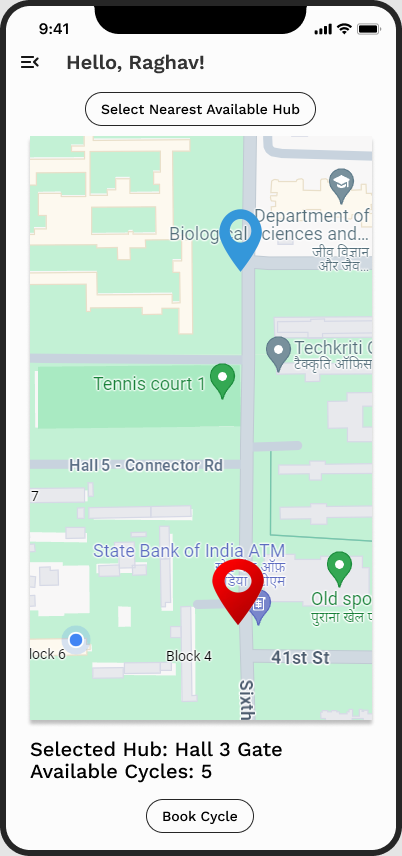
\includegraphics[scale=0.3]{main-ui.png}
    \hspace{30px}
    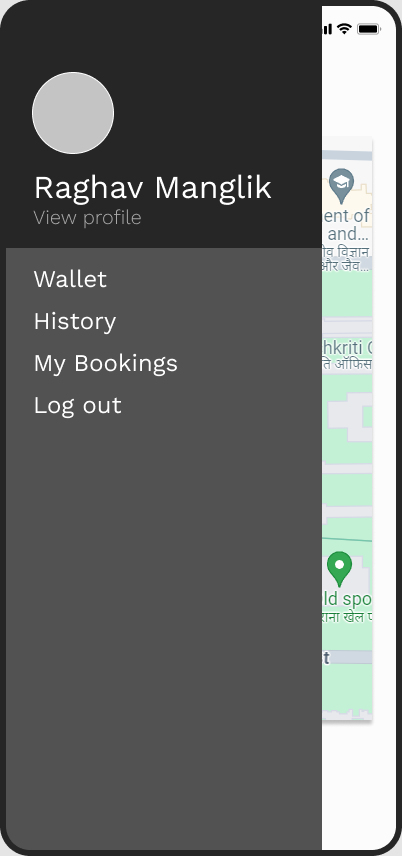
\includegraphics[scale=0.3]{navbar-ui.png}
    \hspace{30px}
    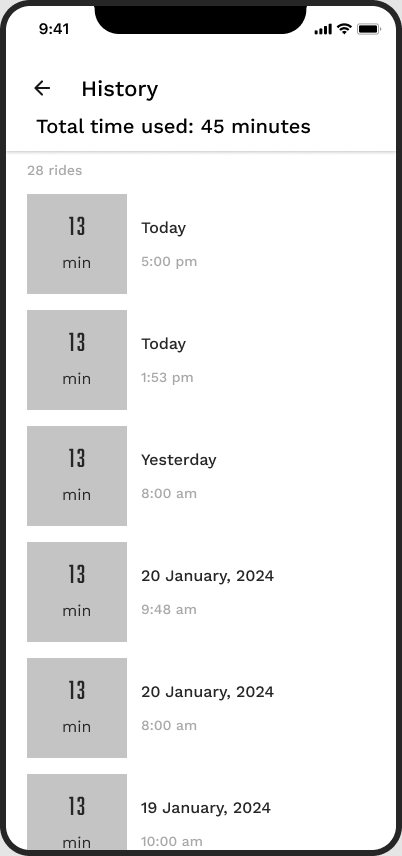
\includegraphics[scale=0.3]{history-ui.png}
\end{figure}

The main screen of the app will present a map view of the campus, with the hubs marked on it. The user can select a hub to view the number of available cycles at that hub. The user can also search for the nearest hub from their location. 

The user can also view their booking history, which will contain details like the hub from which the cycle was booked, the time of booking, the duration of the ride, etc.

The home screen presents several options, such as a profile sidebar that features additional choices like Personal Info, Wallet, History, My Bookings, and a Log Out button. Additionally, the home screen displays the user's preferred hub along with functions for viewing the map and searching for hubs.
\subsubsection{Hardware Interfaces}
\begin{itemize}
    \item \textbf{User devices}: The software would be available for use in devices with internet access, using which the users can directly book their cycles. This will include smartphones, tablets and laptops. Accessibility of the software on mobile devices like smartphones would make the process of cycle booking easy and handy for the user.
    \item \textbf{Cycle Locking mechanism}: The cycle locking mechanism would be made using solenoid locks present at the cycle hubs. The locks will be accessed by the server using an Arduino microcontroller, and its communication will be bridged using the Python \texttt{pyserial} library.
    \item \textbf{Keeping track of parked cycles using RFID}: Each bicycle will be equipped with an RFID tag, and RFID readers will be present at hubs along with each lock. This RFID-based system will keep track of which cycles are parked, enabling a quick and hassle-free cycle issuing and submission system. The unique identification of RFID tags will provide our users with a reliable and convenient solution for renting and returning cycles.
\end{itemize}
\begin{center}
    \includegraphics*[scale=0.75]{rfid-img.png}
\end{center}
\subsubsection{Software Interfaces}
\begin{itemize}
    \item The server-side components, including the database, must be hosted in a Linux-based operating system environment
    \item The client-side components must be functional on modern web browsers as well as their mobile versions, like Google Chrome, Safari, Mozilla Firefox, Microsoft Edge, and Brave
    \item The database management system used by us will be PostgreSQL. The following databases will be created:
    \begin{itemize}
        \item The user database will store all users’ data, including authentication details and personal information
        \item The rides database will store all trips’ data, including the duration and user associated with the trip
        \item The hubs database will store all cycle hubs’ data - number of available cycles and location of the hub
        \item The cycles database will store all cycles’ data - age, location, usability
        \item The payments database will store all the information related to payments
        \item The maintenance database will store the maintenance history of all cycles
        \item The booking database will store all past and future bookings
    \end{itemize}
\end{itemize}

\subsection{Functional Requirements}
\subsubsection{Administrative access using designated usernames and passwords}
\begin{itemize}
    \item Usernames and passwords, known only to authorized users, authenticate their identity during login and grant them administrative access control for system management, including notifying users
    \item Administrative access allows users to authenticate or deactivate user accounts, including resetting passwords and managing user access.
    \item Administrative access allows users to update the inventory of available bicycles, add new bicycles to any operating hub, or remove bicycles that are no longer available
    \item Administrative access allows users to adjust rental and membership prices and see users with negative balances
\end{itemize}

\subsubsection{Provision for users to avail services and subscribe for enhanced features}
\begin{itemize}
    \item The system allows users to create their profiles by providing essential information, password, and identification proof, IITK campus email for campus residents, and contact numbers for visitors
    \item After successful authentication, the system allows users to update their personal information, reset their passwords, and avail of bicycle rental services
    \item The system allows users to become members and avail of enhanced features by paying a monthly subscription fee
\end{itemize}

\subsubsection{Availability of an advance cycle booking system for subscribed users}
\begin{itemize}
    \item Subscribed users gain exclusive access to a bicycle booking system, offering them early access to available bicycles
    \item Subscribed users can define their booking window by providing necessary information such as date, time, and location for their advanced bookings, allowing them to reserve bicycles for a specified period in advance by paying a booking fee charged according to the time for which the bicycle was booked
    \item The system offers flexibility in booking options, allowing subscribed users to modify or cancel their advanced bookings based on their changing plans
\end{itemize}

\subsubsection{Real-time visibility of available cycles at each hub}
\begin{itemize}
    \item The system allows the display of real-time data on available bicycles at each hub
    \item Users can use the map interface integrated into the system, providing a visual representation of cycle hub locations and the number of available bicycles at each site
    \item The system automatically refreshes after a specific time period for real-time updates to ensure that users have the latest information on cycle availability
\end{itemize}

\subsubsection{Visibility of hubs in proximity to any specified location}
\begin{itemize}
    \item The system allows users to input a specific address landmark or use their current location as the basis for finding nearby hubs
    \item The system, if given permission, utilizes location-based services (LBS), like GPS or Wi-Fi positioning, to determine the current location of the user or any specified location
\end{itemize}

\subsubsection{Implementation of a scheduled maintenance system for the upkeep of cycles}
\begin{itemize}
    \item The system defines a regular maintenance schedule for each cycle, considering factors such as total usage time and customers' feedback
    \item The system automatically sends maintenance reminders to maintenance service providers
    \item The system provides customer support for handling emergency maintenance situations, such as breakdowns or safety-related issues
\end{itemize}

\subsubsection{Customer feedback mechanism for maintenance or post-ride experiences}
\begin{itemize}
    \item The system allows users to report any issues with bicycles through the dedicated reporting system
    \item The system defines a feedback form where users can report any issues and give feedback by including fields for specific details, such as cycle ID, Hub location, and/or a description of the problem
    \item The system provides a rating system (5 stars rating system) for users to quickly express their overall satisfaction with the ride and the bicycle itself
\end{itemize}

\subsubsection{Access to detailed analytics, including ride and payment history}
\begin{itemize}
    \item The system provides a user-friendly dashboard where users can access and review detailed analytics of their ride history, including
    \begin{itemize}
        \item Total number of rides
        \item Date and time of each ride
        \item Source and destination of each ride
        \item Duration of each ride
        \item Cost charged for each ride
        \item Average ride duration
    \end{itemize}
    \item The system provides a dashboard where users can access and review detailed analytics of wallet activities of users, including
    \begin{itemize}
        \item Subscription charges (if any)
        \item Current balance
        \item Transcation history
        \item Payment methods used
    \end{itemize}
\end{itemize}

\subsubsection{Implementation of a notification system}
\begin{itemize}
    \item The system sends regular notifications to users to inform them about upcoming maintenance activities or system updates that might affect bike availability
    \item The system sends reminders to users about upcoming subscription renewals
\end{itemize}

\subsection{Use Case Model}
\subsubsection{Use Case 1}
\begin{center}
\includegraphics*[scale=0.5]{usecase-1.png}
\begin{tabular}{|l|p{10cm}|}
    \hline
    \textbf{Author} & Pathe Nevish Ashok \\
    \hline
    \textbf{Purpose} & To let the resident/visitor access cycles from a cycle hub and charge them based on their activity time \\
    \hline
    \textbf{Requirements Traceability} &User should be logged in to the app and should have access to the Internet \\
    \hline
    \textbf{Priority} &The priority of this use case is high as it is the feature of utmost  importance and Is one of the major reasons for making this app \\
    \hline
    \textbf{Pre Conditions} &The user should be physically present at one of the cycle hubs on campus \\
    \hline
    \textbf{Post Conditions} & The user will get access to the desired cycle until they return it to another cycle hub, and they will be charged based on the time of the ride\\
    \hline
    \textbf{Actors} & The actors involved in this use case are the campus residents/visitors who want access to cycles to travel across the campus\\
    \hline
\end{tabular}
\end{center}
\subsubsection{Use Case 2}
\begin{center}
\includegraphics*[scale=0.5]{usecase-2.png}
\begin{tabular}{|l|p{10cm}|}
    \hline
    \textbf{Author} & Raghav Manglik, Srishti Chandra \\
    \hline
    \textbf{Purpose} & To let the user know the availability of cycles at strategically placed different cycle hubs with the help of a campus map \\
    \hline
    \textbf{Requirements Traceability} & The user should be logged in and should give access to  the location if possible\\
    \hline
    \textbf{Priority} & The priority of this use case is medium as it provides a feature for increased convenience and is not highly important for campus residents in particular\\
    \hline
    \textbf{Pre Conditions} &The user should either give location access to the app or select a checkpoint manually from the app \\
    \hline
    \textbf{Post Conditions} & The user will get to know the availability of the cycles in the   nearby/desired cycle hubs\\
    \hline
    \textbf{Actors} & The actors involved in this use case are the campus residents/visitors who want to know the availability of cycles on the campus\\
    \hline
\end{tabular}
\end{center}
\subsubsection{Use Case 3}
\begin{center}
\includegraphics*[scale=0.5]{usecase-3.png}
\begin{tabular}{|l|p{10cm}|}
    \hline
    \textbf{Author} & Anaswar K B \\
    \hline
    \textbf{Purpose} &  To let the user create an account on the portal\\
    \hline
    \textbf{Requirements Traceability} & The user should have a valid ID proof for the administrator to authenticate the user\\
    \hline
    \textbf{Priority} & The priority of this use case is high as if the user does not have an account, they can not use the app\\
    \hline
    \textbf{Pre Conditions} &The user should possess the required details along with an ID proof for the admin to authenticate \\
    \hline
    \textbf{Post Conditions} & An account will be created for the user on the app\\
    \hline
    \textbf{Actors} & The actors involved in this use case are the users who want to create an account on the app and the administrator who authenticates the user\\
    \hline
\end{tabular}
\end{center}
\subsubsection{Use Case 4}
\begin{center}
\includegraphics*[scale=0.5]{usecase-4.png}
\begin{tabular}{|l|p{10cm}|}
    \hline
    \textbf{Author} & Khushi Gupta, Ananya Singh Baghel, Kaneez Fatima\\
    \hline
    \textbf{Purpose} &  To let the user know their previous usage statistics, such as the date of the trip, the duration for which the cycle was accessed, pickup hub, drop hub, etc.\\
    \hline
    \textbf{Requirements Traceability} & The user must have an account on the app\\
    \hline
    \textbf{Priority} &The priority of this use case is medium, as knowing the stats is also an additional feature of this app and not a major feature \\
    \hline
    \textbf{Pre Conditions} & The user must have completed at least one ride using their account on the application\\
    \hline
    \textbf{Post Conditions} & The user will receive the statistics of all the previous rides along with the option to get to know the statistics in a cumulative manner too\\
    \hline
    \textbf{Actors} &The actors involved in this use case are users who want to know their ride statistics \\
    \hline
\end{tabular}
\end{center}
\subsubsection{Use Case 5}
\begin{center}
\includegraphics*[scale=0.5]{usecase-5.png}
\begin{tabular}{|l|p{10cm}|}
    \hline
    \textbf{Author} &  Wadkar Srujan Nitin\\
    \hline
    \textbf{Purpose} & To let the user have a virtual wallet from which the charges will be deducted and allow them to recharge their wallet \\
    \hline
    \textbf{Requirements Traceability} & The user must have an account on the app and also have a UPI/bank account to recharge the wallet\\
    \hline
    \textbf{Priority} & The priority of this use case is high as it is necessary to maintain a digital wallet to pay for the rides\\
    \hline
    \textbf{Pre Conditions} & The user must have created a wallet on the app for the expenses to be deducted from the user’s wallet\\
    \hline
    \textbf{Post Conditions} & The wallet will show the remaining balance or the amount required to pay when a ride is completed, when the wallet is recharged, or whenever the user demands\\
    \hline
    \textbf{Actors} & The actors involved in this use case are users for whom the wallet is maintained and the admin\\
    \hline
\end{tabular}
\end{center}
\subsubsection{Use Case 6}
\begin{center}
\includegraphics*[scale=0.5]{usecase-6.png}
\begin{tabular}{|l|p{10cm}|}
    \hline
    \textbf{Author} & Debraj Karmakar, Amogh Bhagwat\\
    \hline
    \textbf{Purpose} & To let the user give feedback about the cycles as well as the app experience after the ride \\
    \hline
    \textbf{Requirements Traceability} & The user must have an account on the app and must have used the app for a sufficient amount of time\\
    \hline
    \textbf{Priority} & The priority of this use case is medium, as maintenance of cycles will not be fully dependent on feedback and comprehensive testing of the app will be done to ensure no bugs are found by the user\\
    \hline
    \textbf{Pre Conditions} & The user should have checked the condition of the cycle at the time of giving feedback about it as well as they should have used the app for a sufficient amount of time\\
    \hline
    \textbf{Post Conditions} & The app will record the feedback of the user and the admin will take actions by viewing the feedback if necessary\\
    \hline
    \textbf{Actors} & The actors involved in this use case are the users who will provide the feedback to the app and the admin who will view it\\
    \hline
\end{tabular}
\end{center}

\newpage
\section{Other Non-Functional Requirements}
\subsection{Performance Requirements}
The software should maintain a 99.9\% uptime, allowing users to access cycle rental services without significant disruptions, excluding scheduled maintenance windows.

The system should support a minimum of 500 concurrent rental transactions per minute to ensure efficient and timely processing of user requests.The system should respond to user requests for cycle rentals within 3 seconds under normal operating conditions.The software should be designed with built-in fault tolerance mechanisms to mitigate the impact of hardware or software failures, ensuring uninterrupted service availability.

\subsection{Safety and Security Requirements}
\begin{itemize}
    \item \textbf{User Authentication}: The system must employ robust user authentication mechanisms, such as strong password policies or multi-factor authentication, to verify the identity of users before granting access to rental services. Proper login mechanisms should be used to avoid hacking.
    \item \textbf{Data Encryption}: All sensitive user information, including personal details and payment data, must be encrypted during transmission to prevent unauthorized access and data breaches. Information should be securely transmitted to the server without any changes in information. Secure storage of passwords will be done after salting and hashing the passwords. In other words, the system admin can only verify if the password is correct but won’t know what the password submitted by the user was. On maintenance complaints, the cycle’s information will be sent to the admin. The complainant users’ information is not sent to the server.
    \item \textbf{Secure Transactions}: Payment transactions within the software must be conducted through secure channels. The API of a safe payment gateway, like Razorpay, will be used for the same. A notification will be sent to the concerned people whenever a transaction is added.
    \item \textbf{Physical Security}: Implement physical security measures for any hardware components of the system to prevent unauthorized access. The cycle locks will only be opened when the user scans the QR code on the cycle.
\end{itemize}

\subsection{Software Quality Attributes}
\subsubsection{Usability}
\begin{itemize}
    \item \textbf{Intuitiveness}: The software should have a user-friendly interface, allowing users to navigate through the rental process without confusion easily.
    \item \textbf{Response Time}: Provide quick response times for user interactions, such as renting a cycle or viewing available options.
\end{itemize}

\subsubsection{Availability}
\begin{itemize}
    \item In case of a server crash, the system state must be restored within two hours.
    \item \textbf{Performance Scalability}: The number of users will increase in large numbers during campus fests. The system availability needs to be enough for this purpose. Ensure the software can handle an increased load as the user base grows.
\end{itemize}
\subsubsection{Reliability}
\begin{itemize}
    \item The MTTF (mean time to failure) shall be more than one week.
    \item The system must undergo extensive feature testing, load testing, and regression testing prior to release and/or deployment.
    \item The system should be reliable in giving correct results consistently.
\end{itemize}

\subsubsection{Portability}
We are using Django with bootstrap and inline CSS to design the front-end part of our application, thus our application is portable, responsive and can run on most of the modern web browsers.

\newpage
\section{Other Requirements}

\newpage
\section{Data Dictionary}

\newpage
\section{Group Log}
\end{document}